\documentclass{beamer}
\usepackage[utf8]{inputenc}
\usepackage{natbib}
\usepackage{graphicx}
%\usepackage{natbib}
\usepackage{graphicx}
\usepackage{tikz}
\usepackage[T1]{fontenc}    % better to have fontenc *before* inputenc
\usepackage[utf8]{inputenc}

\usepackage[english]{babel}
\usetikzlibrary{arrows,decorations.markings}
\usetikzlibrary{arrows.meta}% CVS


% \newtheorem{problem}{Problem}
% \newtheorem{attempt}{Attempt}
% \newtheorem{theorem}{Theorem}[section]
% \newtheorem{corollary}{Corollary}[theorem]
% \newtheorem{lemma}[theorem]{Lemma}
% \newtheorem{proposition}[theorem]{Proposition}
% \theoremstyle{definition}
% \newtheorem{definition}{Definition}[section]
% %\theoremstyle{indented}
% \newtheorem*{remark}{Remark}
% \newenvironment{titlemize}[1]{%
%   \paragraph{#1}
%   \begin{itemize}}
%   {\end{itemize}}
  
% \theoremstyle{definition}
% \newtheorem{example}{Example}[section]  
% \theoremstyle{definition}
% \newtheorem{exercise}{Exercise}[section]  


\usetheme{Madrid}
\usecolortheme{default}

%------------------------------------------------------------
%This block of code defines the information to appear in the
%Title page
\title %optional
{Combinatorics of stability conditions}

% \subtitle{A short story}

\author % (optional)
{Rhys Wells}

\institute % (optional)
{
Liverpool University
}

\date % (optional)
{\today}


%End of title page configuration block
%------------------------------------------------------------



%------------------------------------------------------------
%The next block of commands puts the table of contents at the 
%beginning of each section and highlights the current section:

\AtBeginSection[]
{
  \begin{frame}
    \frametitle{Table of Contents}
    \tableofcontents[currentsection]
  \end{frame}
}
%------------------------------------------------------------


\begin{document}

%The next statement creates the title page.
\frame{\titlepage}


%---------------------------------------------------------
%This block of code is for the table of contents after
%the title page
% \begin{frame}
% \frametitle{Table of Contents}
% \tableofcontents
% \end{frame}
%---------------------------------------------------------

% Done
\section{Introduction}

\begin{frame}{Today's Discussion}

Today I am going to discuss the combinatorics of stability conditions of elements of fine compactified Jacobians, over a single stable curve in the case of line bundles. \pause  In particular it is enough to consider the stability of divisors on the graph $G$ of curve it is over.\\\pause

% Nodes on the curve correspond to edges.

~\\

For a graph $G$, I am going to\\ 
~\\

\begin{itemize}
    \item define the notion of a $\phi$-stability condition, $\sigma_{\phi}(G)$, and give examples \pause

\item to introduce the notion of a generalised stability $\sigma(G)$ condition \pause

\item and propose a question relating $\sigma_{\phi}(G)$ and $\sigma(G)$.
\end{itemize}

\end{frame}

% Done
\section{$\phi$-stability}

\begin{frame}{Notation}

Define the stability space to be $V(G) \subseteq \mathbb{R}^{Vert(G)}$ such that for $\phi \in \mathbb{R}^{Vert(G)}$ we have $\sum_{i \in Vert(G)} \phi_i =0$ and let $S(G) =Div^{0}(G) \subseteq V(G)$.\\ \pause

% introduced in \cite{oda1979compactifications}

\skipline
\begin{definition}
Let $\phi \in V(G)$, we say $d \in S(G)$ is $\phi$-(semi) stable if,

\begin{equation*}\label{stabinequal}
\Bigl| \sum_{v \in Vert(G_0)} d(v) - \phi(v)\Bigr| \underset{(\le)}{<}  \frac{\# (E(G\setminus G_0) \cap E(G\setminus G_0^{c}) )}{2},
\end{equation*}

for all $\emptyset \subsetneq G_0 \subsetneq G $, where $G_0$ is a complete subgraph ($G_0^{c}$ denotes the complete subgraph with complement vertices to $G_0$).
\end{definition}\pause

\skipline 

\\By removing degenerate hyperplanes let $Q_G$ denote the set of convex polytopes of $V(G)$. And the set of $\phi$-stability conditions is given by,
$$\sigma_{\phi}(G):=\{d : \text{Vert}(G) \rightarrow \mathbb{Z} \mid \phi \text{-stable}\} \subseteq S(G).$$


% remark on when $\phi$ is non-degenerate. 

\end{frame}

\begin{frame}{Illustrative examples}

Let $G$ be

\begin{center}
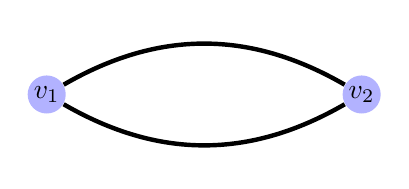
\begin{tikzpicture}[main_node/.style={circle,fill=blue!30,minimum size=1em,inner sep=1pt]}]

    \node[main_node] (1) at (0,0) {$v_1$};
    \node[main_node] (2) at (4, 0)  {$v_2$};


    \path[-,draw,ultra thick]
    (1) edge[bend left] node [] {} (2)
    (2) edge[bend left] node [right] {} (1);
    
%   \path[every node/.style={font=\sffamily\Large}]
%     (1) edge[bend left] node [] {} (2)
%     (2) edge[bend left] node [right] {} (1);
\end{tikzpicture}
\end{center} 

and let $\phi=(\frac{1}{3},-\frac{1}{3}) \in V(G)$, what is $\sigma_{\phi}(G)$?\\\pause
~\\

Take $\underline{d}=(d,-d) \in S(G)$ then we have $\bold{d}$ is $\phi$-stable if

$$|d-\frac{1}{3}|<1.$$

\begin{center}
    \begin{tikzpicture}[xscale=2.5]
\draw[-][draw=very thick] (-2,0) -- (2,0);
\draw [thick] (-1,-.1) node[below]{-1} -- (-1,0.1);
\draw [thick] (0,-.1) node[below]{0} -- (0,0.1);
\draw [thick] (0.3,-.1) node[below]{$\phi=\frac{1}{3}$} -- (0.3,0.1);
\draw [thick] (1,-.1) node[below]{1} -- (1,0.1);
\draw [thick,red] (-0.7,-.1) node[below]{$-\frac{2}{3}$} -- (-0.7,0.1);
\draw [thick,red] (1.3,-.1) node[below]{$\frac{4}{3}$} -- (1.3,0.1);
\end{tikzpicture}
\end{center} \pause

Therefore we have $\sigma_{\phi}(G) = \{(0,0),(1,-1)\}.$ 

% A spanning tree is a subset of Graph G, which has all the vertices covered with minimum possible number of edges.

\end{frame}

\begin{frame}

Similarly let $G$ be,

\begin{center}
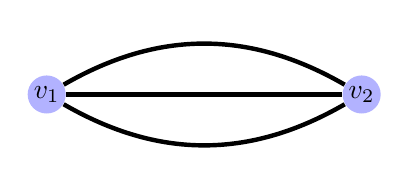
\begin{tikzpicture}[main_node/.style={circle,fill=blue!30,minimum size=1em,inner sep=1pt]}]

    \node[main_node] (1) at (0,0) {$v_1$};
    \node[main_node] (2) at (4, 0)  {$v_2$};


    \path[-,draw,ultra thick]
    (1) edge[bend left] node [] {} (2)
    (2) edge[bend left] node [right] {} (1)
    (2) edge[] node [right] {} (1);
    
%   \path[every node/.style={font=\sffamily\Large}]
%     (1) edge[bend left] node [] {} (2)
%     (2) edge[bend left] node [right] {} (1);
\end{tikzpicture}
\end{center}

This time we have 
$$|d-\frac{1}{3}|<\frac{3}{2}.$$

\begin{center}
    \begin{tikzpicture}[xscale=2]
\draw[-][draw=very thick] (-3,0) -- (3,0);
\draw [thick] (-1,-.1) node[below]{-1} -- (-1,0.1);
\draw [thick] (-2,-.1) node[below]{-2} -- (-2,0.1);
\draw [thick] (0,-.1) node[below]{0} -- (0,0.1);
\draw [thick] (0.3,-.1) node[below]{$\phi=\frac{1}{3}$} -- (0.3,0.1);
\draw [thick] (1,-.1) node[below]{1} -- (1,0.1);
\draw [thick] (2,-.1) node[below]{2} -- (2,0.1);
\draw [thick,red] (-1.3,-.1) node[below]{$-\frac{7}{6}$} -- (-1.3,0.1);
\draw [thick,red] (1.83,-.1) node[below]{$\frac{11}{6}$} -- (1.83,0.1);
\end{tikzpicture}
\end{center}\pause

and so $\sigma_{\phi}(G) = \{(0,0),(1,-1),(-1,1)\}.$\\\pause

~\\

For $\phi$ non-degenerate the elements of $\sigma_{\phi}(G)$ are close to $\phi$ and there are $|\sigma_{\phi}(G)|=|\#\text{Spanning trees of G} |$ many.


\end{frame}

\section{Generalised stability}

% Done
\begin{frame}{Chip firing and $J(G)$}

We will now introduce an abstract notion of stability which is not reliant on the polarisation $\phi$. In order to define it I will need a detour into algebraic graph theory to define the Jacobian of a graph by the chip-firing equivalence.\\  \pause
% \linebreak
% \vfill
~\\
Let $G$ be a labelled multigraph with genus $g=b_1(G)$.
Divisors $D , D^{'} \in Div(G)$ are equivalent is related by  a by a chip-firing procedure. Where one fires from a vertex $v$ on $D$ to obtain $D^{'}$ by mapping $D$ to 

$$D^{'}= D - deg(v) \cdot v+\sum_{vw\in E} w.$$  

  \begin{center}
 
  
        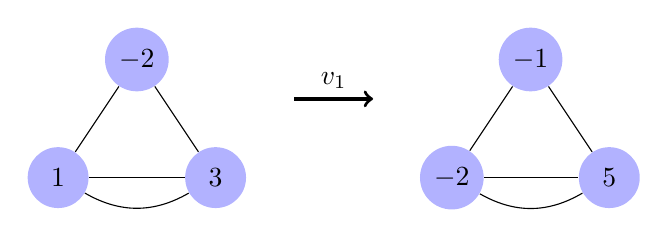
\begin{tikzpicture}[main_node/.style={circle,fill=blue!30,minimum size=2.2em,inner sep=3pt]}]

    \node[main_node] (1) at (0,0) {$-2$};
    \node[main_node] (2) at (-1, -1.5)  {$1$};
    \node[main_node] (3) at (1, -1.5) {$3$};
    
  \path[every node/.style={font=\sffamily\small}]
    (1) edge node [] {} (2)
    % (1) edge[bend left] node [] {} (2)
    (2) edge node [] {} (3)
    (3) edge node [] {} (1)
    (3) edge[bend left] node [] {} (2);

    % (3) edge[bend right] node [left] {} (2);
    
        \node[main_node] (a) at (5,0) {$-1$};
    \node[main_node] (b) at (4, -1.5)  {$-2$};
    \node[main_node] (c) at (6, -1.5) {$5$};
    
  \path[every node/.style={font=\sffamily\small}]
    (a) edge node [] {} (b)
    % (1) edge[bend left] node [] {} (2)
    (b) edge node [] {} (c)
    (c) edge node [] {} (a)
    (c) edge[bend left] node [] {} (b);
    
     \draw [-to,very thick](2,-0.5) -- (3,-0.5);
     \draw [thick] (2.5, -0.5) node[above]{$v_1$} -- (2.5, -0.5);
\end{tikzpicture}
  \end{center}
  
%   There is also the reverse action
  
  \end{frame}
  
% Done
\begin{frame}

Linear combinations of chip-firings are called a firing script and the set of firing scripts is denoted by $\mathbb{Z}^{Vert(G)}$.\\ \pause

% Note the total degree stays the same.

~\\
There exists a homomorphism $L:\mathbb{Z}^{Vert(G)} \rightarrow Div(G)$ which assigns to each script a divisor by the mapping,

$$L=Deg - Adj^{T}$$

For the graph,

\begin{center}
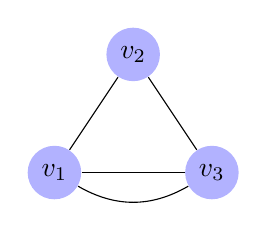
\begin{tikzpicture}[main_node/.style={circle,fill=blue!30,minimum size=1em,inner sep=3pt]}]

    \node[main_node] (1) at (0,0) {$v_2$};
    \node[main_node] (2) at (-1, -1.5)  {$v_1$};
    \node[main_node] (3) at (1, -1.5) {$v_3$};
    
  \path[every node/.style={font=\sffamily\small}]
    (1) edge node [] {} (2)
    % (1) edge[bend left] node [] {} (2)
    (2) edge node [] {} (3)
    (3) edge node [] {} (1)
    (3) edge[bend left] node [] {} (2);

    % (3) edge[bend right] node [left] {} (2);

\end{tikzpicture}
\end{center}

we have the Laplacian 

$$ L=
\begin{pmatrix}
3 & -1 & -2\\
-1 & 2 & -1\\
-2& -1& 3 
\end{pmatrix}
$$

\end{frame}
% Done
\begin{frame}

Define $\tilde{L}$ by deleting the associated row and columns of $L$ of a single vertex.\\ 

$$ L=
\begin{pmatrix}
3 & -1 & -2\\
-1 & 2 & -1\\
-2& -1& 3 
\end{pmatrix}
$$
    
We define $J(G):=S(G)/ Im(\tilde{L})$ by the cokernel of $\tilde{L}$.\pause

~\\
The matrix-tree theorem in particular gives a bijection between the number of spanning trees and the order of $Jac(G)$ and it can be shown that $|Jac(G)|=det(\tilde{L})$. For

\begin{center}
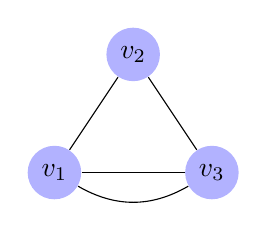
\begin{tikzpicture}[main_node/.style={circle,fill=blue!30,minimum size=1em,inner sep=3pt]}]

    \node[main_node] (1) at (0,0) {$v_2$};
    \node[main_node] (2) at (-1, -1.5)  {$v_1$};
    \node[main_node] (3) at (1, -1.5) {$v_3$};
    
  \path[every node/.style={font=\sffamily\small}]
    (1) edge node [] {} (2)
    % (1) edge[bend left] node [] {} (2)
    (2) edge node [] {} (3)
    (3) edge node [] {} (1)
    (3) edge[bend left] node [] {} (2);

    % (3) edge[bend right] node [left] {} (2);

\end{tikzpicture}
\end{center}

we have $Jac(G)=\mathbb{Z}_5$.
    
\end{frame}

% Done
\begin{frame}{Class representatives for $J(G)$}

Let $\pi: S(G) \rightarrow J(G)$ be the quotient map of $\tilde{L}$.\\ 
~\\

We say a set $\sigma(G) \subseteq S(G)$ denotes a set of class representatives for $J(G)$ in $S(G)$.\\ 

~\\
If for all $c \in S(G)$ there exists a unique $d \in \sigma(G) $ such that $c-d \in Im(\tilde{L})$. Equivalently $\sigma(G)$ is a section of $\pi$.\\ \pause

% , $c=\tilde{L}(f)+d \in S(G)$ and equivalently

\begin{center}
\begin{tikzpicture}[main_node/.style={circle,fill=blue!30,minimum size=1em,inner sep=1pt]}]

    \node[main_node] (1) at (0,0) {$v_1$};
    \node[main_node] (2) at (4, 0)  {$v_2$};


    \path[-,draw,ultra thick]
    (1) edge[bend left] node [] {} (2)
    (2) edge[bend left] node [right] {} (1)

    
%   \path[every node/.style={font=\sffamily\Large}]
%     (1) edge[bend left] node [] {} (2)
%     (2) edge[bend left] node [right] {} (1);
\end{tikzpicture}
\end{center}

The chip-firing at $v_1$ we get $(d,-d) \in \mathbb{Z}^{2}$ sent to $(d-2,d+2)$ so if $d$ is odd it remains odd, similarly if it is even then it remains even. \\  

~\\
Therefore $\sigma(G)$ could be  either $\{(0,0),(1,-1)\}$ or  $\{(1,-1), (4,-4)\}$ however the latter case is not close together unlike $\sigma_{\phi}(G)$.
    
\end{frame}

% Done
\begin{frame}{Free and transitive action}

If we define $\sigma(G)$ to be a complete set of representatives so it admits a action by translating by elements of $J(G)$, which is free and transitive.\\ \pause
 
 ~\\
 
Recall $\pi: S(G) \rightarrow J(G)$ and let $e \in S(G)$ be such that $\pi(e)=g$, then we have the following action
\begin{align*}
    \beta: Jac(G) \times \sigma(G) &\rightarrow S(G)\\
    (g,d) & \mapsto \text{The unique element of $\sigma(G)$ that represents $e+d$ }.
\end{align*}

As this is free and transisitve so we have $|\sigma(G)|=|J(G)|=|\# \text{ Spanning trees}|$ which is finite and agrees with what we saw in the $\sigma_{\phi}(G)$ case. 
\end{frame}
 
% Done 
\begin{frame}{Proximity}
    
By studying $\sigma_{\phi}(G)$ we require the divisors of a generalise stability condition to be near each other.\\ 

~\\
To define a notion of proximity we consider the set of divisors IBD which is derived from taking a  fixed spanning tree and adding $1$ to the endpoints of $G\setminus \Gamma$ in all possible ways.\\  
~\\\pause

More formally denote the set of orientations of $G \setminus \Gamma$ to be the set $S=\{s:Edges(G \setminus \Gamma) \rightarrow Vert(G)$\} and let IBD be,

 $$IBD:= \{ d \in S^{g}(G)  \mid d= \sum_{l \in E(G\setminus \Gamma)} \delta _{s(l)} \text{ for all } s \in S  \}.$$

\end{frame}

% Done
\begin{frame}

For example let,

\begin{center}
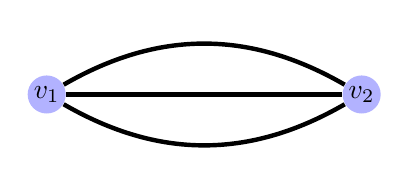
\begin{tikzpicture}[main_node/.style={circle,fill=blue!30,minimum size=1em,inner sep=1pt]}]

    \node[main_node] (1) at (0,0) {$v_1$};
    \node[main_node] (2) at (4, 0)  {$v_2$};


    \path[-,draw,ultra thick]
    (1) edge[bend left] node [] {} (2)
    (2) edge[bend left] node [right] {} (1)
    (2) edge[] node [right] {} (1);
    
%   \path[every node/.style={font=\sffamily\Large}]
%     (1) edge[bend left] node [] {} (2)
%     (2) edge[bend left] node [right] {} (1);
\end{tikzpicture}
\end{center}

we have $IBD=\{(2,0),(1,1),(0,2)\}.$\pause

To remain in the total degree zero case we shift back by letting 

$$S^{-g}(G)=\{d^{'} \in \mathbb{Z}^{Vert(G)} \mid \sum d^{'}(v) = -g\}.$$ 

For a fixed $\Gamma_i$ we denote the set of divisors near $d^{'} \in S^{-g}(G)$ to be,

$$\sigma^{'}(\Gamma_i,d^{'}
):= \{ d \in S(G) \mid d= d^{'} + \sum_{l \in E(G\setminus \Gamma_i)} \delta _{s(l)} \text{ for all } s \in S  \}.$$

\end{frame}

% Done
\begin{frame}{Generalised stability definition}

We are now ready to define a generalised stability condition.\\ 
~\\
We wish our definition to be a set of class of representatives for $J(G)$ and are near each other as discussed. \pause

\begin{definition}\label{axioms12}
A generalised stability condition for $G$ is a subset $\sigma(G) \subseteq S(G)$ such that,

\begin{enumerate}
    \item the set $\sigma(G)$ is a complete set of representatives for the action of $J(G)$ \pause
    
\item and for each spanning tree $\Gamma_i$ there exists $d_i^{'} \in S^{-g}(G)$ such that 

$$\sigma(G) = \bigcup_{i\in I} \sigma^{'}(\Gamma_i,d_{i}^{'}).$$ 

\end{enumerate}
\end{definition}

\end{frame}

% Done
\begin{frame}{Example}
Take 

\begin{center}
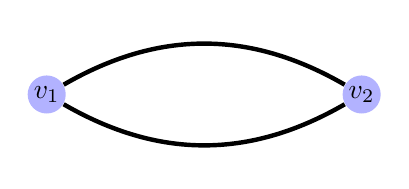
\begin{tikzpicture}[main_node/.style={circle,fill=blue!30,minimum size=1em,inner sep=1pt]}]

    \node[main_node] (1) at (0,0) {$v_1$};
    \node[main_node] (2) at (4, 0)  {$v_2$};


    \path[-,draw,ultra thick]
    (1) edge[bend left] node [] {} (2)
    (2) edge[bend left] node [right] {} (1);
    
%   \path[every node/.style={font=\sffamily\Large}]
%     (1) edge[bend left] node [] {} (2)
%     (2) edge[bend left] node [right] {} (1);
\end{tikzpicture}
\end{center} 

We have $IBD=\{(0,1),(1,0)\}$ \\\pause

~\\

If we let $d^{'} \in S^{-1}(G)$ be $(-1,0)$ then we have

$$\sigma(G) = \{(0,0),(1,-1)\}.$$

Similarly for $(0,-1)$.  \pause

We have already seen this can be obtained by letting $\phi=(\frac{1}{3},-\frac{1}{3})$ in which case we have $\sigma_{\phi}(G)=\sigma(G)$.

\end{frame}

% Done for now, needs checked
\section{Research Question}

\begin{frame}{Is there always a $\phi$?}

For an arbitrary graph $G$, let $\Sigma_G$ be the set of generalised stability conditions $\sigma(G)$.\\ 

~\\

Are there generalised stability conditions $\sigma(G)$ that are not $\phi$-stability conditions $\sigma_{\phi}(G)$ for some $\phi$?\\\pause

~\\

Do we always have $\sigma_{\phi}(G)=\sigma(G)$?\\ \pause

~\\

More precisely is the map 

\begin{align*}
    \psi_G: Q_G &\rightarrow \Sigma_G\\
    \phi \in P &\mapsto \sigma_{\phi}(G) 
\end{align*}

surjective? 

\end{frame}


\end{document}